\documentclass[xcolor=svgnames,10pt]{beamer}

%%%%%%%%%%%%%%%%%%%%%%%%%%%%%%%%%%%%%%%%%%%%%%%%%%%%%%%
%%%%%%%%%%%%%%%%%%%%%%%% packages %%%%%%%%%%%%%%%%%%%%%
\usepackage{xepersian}
\settextfont{Yas.ttf}
\defpersianfont\nas[Scale=1.7]{IranNastaliq.ttf}
\defpersianfont\titr{BTitr.ttf}

%%%%%%%%%%%%%%%%%%%%%%%%%%%%%%%%%%%%%%%%%%%%%%%%%%%%%%%
%%%%%%%%%%%%%%%%%%%%%%%% theme %%%%%%%%%%%%%%%%%%%%%%%%
\usetheme{Madrid} % Clean and professional layout

% ---------- Modern color palette ----------
\definecolor{PrimaryNavy}{HTML}{0B3C5D}  % deep blue
\definecolor{AccentTeal}{HTML}{007C7C}   % teal
\definecolor{ExampleGreen}{HTML}{2E8B57} % green for examples
\definecolor{AlertOrange}{HTML}{E67E22}  % orange for alerts
\definecolor{SoftGray}{HTML}{F5F7FA}     % light background
\definecolor{Muted}{HTML}{6B6B6B}        % muted text

% ---------- Color theme configuration ----------
\setbeamercolor{background canvas}{bg=SoftGray}
\setbeamercolor{normal text}{fg=PrimaryNavy}

\setbeamercolor{frametitle}{fg=PrimaryNavy,bg=SoftGray}
\setbeamerfont{frametitle}{series=\bfseries,size=\large}

\setbeamercolor{structure}{fg=AccentTeal}

\setbeamercolor{block title}{fg=white,bg=AccentTeal}
\setbeamercolor{block body}{fg=PrimaryNavy,bg=white}

\setbeamercolor{block title alerted}{fg=white,bg=AlertOrange}
\setbeamercolor{block body alerted}{fg=PrimaryNavy,bg=white}

\setbeamercolor{block title example}{fg=white,bg=ExampleGreen}
\setbeamercolor{block body example}{fg=PrimaryNavy,bg=white}

\setbeamertemplate{navigation symbols}{} % remove navigation buttons
\setbeamertemplate{footline}[frame number] % show only slide number

%%%%%%%%%%%%%%%%%%%%%%%%%%%%%%%%%%%%%%%%%%%%%%%%%%%%%%%
%%%%%%%%%%%%%%%%%%%%%% Paths %%%%%%%%%%%%%%%%%%%%%%%%%%%
\graphicspath{{./Fig/}}

%%%%%%%%%%%%%%%%%%%%%%%%%%%%%%%%%%%%%%%%%%%%%%%%%%%%%%%
%%%%%%%%%%%%%%%%%%%%%% Title %%%%%%%%%%%%%%%%%%%%%%%%%%%
\title{\titr عنوان اسلاید}
\subtitle{زیرعنوان اسلاید}
\author{نام نویسنده}
\institute{نام موسسه}
\date{تاریخ}

%%%%%%%%%%%%%%%%%%%%%%%%%%%%%%%%%%%%%%%%%%%%%%%%%%%%%%%
%%%%%%%%%%%%%%%%%%%% Begin Document %%%%%%%%%%%%%%%%%%%%
\begin{document}

% ---------- Intro slide ----------
\begin{frame}[plain,noframenumbering]
\centering
\vspace{1cm}
{\nas بسم‌الله‌الرحمن‌الرحیم}
\end{frame}

% ---------- Title slide ----------
\begin{frame}
\titlepage
\end{frame}

%%%%%%%%%%%%%%%%%%%%%%%%%%%%%%%%%%%%%%%%%%%%%%%%%%%%%%%
%%%%%%%%%%%%%%%%%%%% Sample Frame %%%%%%%%%%%%%%%%%%%%%%
\section{بخش اول}
\subsection{محیط ریاضی}

\begin{frame}[t]{{\titr عنوان اسلاید با فونت تیتر}}
\begin{flushright}
در این اسلاید محیط‌های قضیه، مثال، اثبات و نتیجه بیان شده است.
می‌توان از محیط \lr{flushright} برای مطالب راست‌چین و از محیط \lr{flushleft} برای مطالب چپ‌چین استفاده نمود تا نمایش مطالب دقیق‌تر باشد.
\end{flushright}

\pause
\begin{theorem}
قضیه
\end{theorem}

\pause
\begin{example}
مثال
\end{example}

\pause
\begin{proof}
اثبات
\end{proof}

\pause
\begin{corollary}
نتیجه
\end{corollary}
\end{frame}

%%%%%%%%%%%%%%%%%%%%%%%%%%%%%%%%%%%%%%%%

\begin{frame}[t]{{\titr استفاده از شکل}}
	\begin{flushright}
فرمت شکل زیر پی دی اف میباشد:
	\end{flushright}
	\begin{figure}
		\centering
		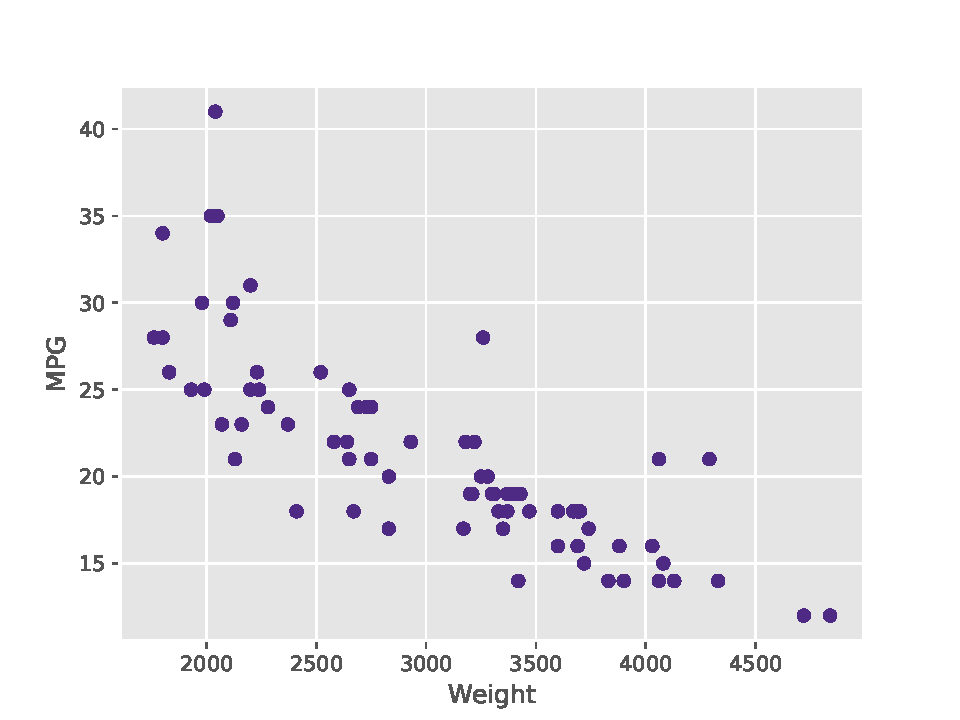
\includegraphics[width=0.6\textwidth]{plot-python.pdf}
		\caption{نمودار یچیزی}
		\label{fig:graph-python}
	\end{figure}
\end{frame}

\begin{frame}[plain,noframenumbering]
\centering
\vspace{1cm}
{\nas سوال؟}
\end{frame}

\end{document}
